\chapter{推荐系统综述}

	\section{引言}
		当今的时代是信息过载(Information overload)的时代\citep{info-overload}。对于一个用户来讲互联网上充斥着大量对其无用的信息,如何从这些信息里找到用户感兴趣的信息,并把这些信息推送给用户是推荐系统面临的主要问题。推荐系统通过对用户的历史行为进行挖掘,对用户画像进行建模预测用户未来的行为。

		推荐系统的研究和很多早期的研究相关,比如认知科学(cognitive science)\citep{cognitive-science},信息检索(information retrieval)和预测理论\citep{Forecast-principle}。随着互联网的兴起,研究人员开始研究如何利用用户对物品行为数据来预测用户的兴趣并给用户做推荐\citep{cf-sn}。推荐系统开始成为一个比较独立的研究问题。到2006年为止推荐系统的研究主要集中在基于邻域的协同过滤算法,目前工业界应用最广泛、最知名的算法应该就是亚马逊开发并使用的协同过滤算法\citep{Amazon-cf}。

		近年来很多研究人员意识到推荐的时效性和多样性对于用户的体验度非常重要,而长尾效应对提高商品销售量有非常大的帮助。创建用户兴趣画像则是其中比较有效的解决途径之一,因为度量用户对物品的喜好不仅取决于用户的喜好和物品的属性,也取决于用户所处的环境,或者称做上下文(Context),上下文信息有很多类型,其中时间是一种重要的上下文信息,用户在不同的时间可能喜欢不同的物品,物品在不同的时间也有不同的流行度。因此推荐系统应该是一个动态系统,随着时间的变化会给用户不同的推荐结果\citep{temporal-cf}。

	\section{推荐系统的算法模块}
		\subsection{协同过滤算法}
		协同过滤的根本原理是,人们可以从和自己有相同品味、习性的人群那里获得高质量的推荐。协同过滤算法主要研究如何聚类具有相似兴趣特征的人群并基于此做出推荐,因为算法本身是基于用户社交群体,因此往往会涉及到大规模的用户行为数据的计算。协同过滤的应用领域也很广:电子商务,金融信贷,搜素引擎,互联网企业,网络社区等需要对用户提供个性化体验的服务商。因为中国现有的人口国情,协同过滤算法往往需要面对亿万级用户和海量的用户-主题交互数据。作为输入数据,一个用户是以一个N维度的向量来表示,N代表所有的主题数量。向量内容可以为正也可为负,分别表示了用户喜欢、讨厌该主题的程度。对于热门主题,给其打分的用户会很多,其分数应该乘以一个因子u得到有效的分数,u代表所有给其打分的用户个数的倒数,大多数用户向量是稀疏的。在协同过滤算法中关键性的一步就是要选择测量的距离,描述集合相似度算法有欧氏距离、闵可夫斯基距离、汉明距离等,这里选择余弦距离公式(cosine similiarity),公式描述如下,
		其中$similarity_{uv}$代表用户u与v之间的兴趣相似度,N(u)表示用户u曾经喜欢过的物品集合,N(v)表示用户v曾经喜欢过的物品集合。

		\begin{equation}
			similarity_{uv} = \frac{|N(u)\cdot N(v)|}{||N(u)||\cdot||N(v)||}
			\label{cosine-similiarity}
		\end{equation}
		\\然后利用相似度算法把用户分类成独立的集合,每个用户有且只属于其中的一个集合,对于每个集合,取这个集合最受欢迎的top K 个主题,作为推荐内容推荐给集合的所有用户。大多数情况下协同过滤算法面都临着一个问题:最坏情况下需要遍历所有的用户和所有的主题,算法计算复杂度为O(MN),M是用户数N是主题数,解决方法可以借助一种简单的降维思想加以解决:通过去掉那些非常冷门的主题对N做降维,通过去掉那些非常不活跃的用户对M做降维,计算维度下降的代价是降低了推荐系统的准确性。

		User-Based CF更多的是挖掘用户之间的社交属性,而Item-Based CF更多的是挖掘物品之间的特征属性。根据电子商务业务的特殊性这里选择用Item-Based CF算法,原因包括:
		\begin{itemize}
		\item 现有电子商务的矩阵计算一台服务器即可承受;相反,百万级别的用户,计算量需要用一个spark集群完成计算,从经济效益的角度讲不可取。
		\item 电子商务一般来讲周上线不足100多款,周更新不到5\%,且可以利用增量计算方法更新item-item矩阵;相反,主题用户周增加量为十万数量级,加上用户兴趣、社交、互动的动态变化,增量计算无能为力,导致每次更新user-user矩阵的时候计算量很大。
		\item 如果用ItemCF,会只推荐与相似领域的主题的东西给用户,这样在有限的推荐列表中就可能包含了一定数量本领域不热门的item,所以ItemCF推荐长尾的能力比较强,代价是推荐多样性不足,但是对整个系统而言,因为不同的用户的主要兴趣点不同,所以系统的coverage也会很大。
		\item ItemCF的算法还可以为推荐结果做出理性的解释。如一个用户之前购买过魔兽世界的主题包,推荐系统会给其推荐魔兽争霸主题包并附上说明:因为用户曾经买过类似的主题包,并且评价分数不错。
		\end{itemize}

		\subsection{聚类模型算法}
		聚类分析(Cluster analysis)是对于统计数据分析的一门技术,和分类算法一个主要的区别就是聚类不需要人工参与打标签,基于聚类和SlopeOne预测的协同过滤方法,也可以在一定程度上解决传统协同过滤算法用户评分矩阵稀疏和冷启动问题,在降低用户评分矩阵稀疏性的同时提高目标用户最近邻居的查询速度。聚类是把相似的对象通过静态分类的方法分成不同的组别或者更多的子集(subset),这样让在同一个子集中的成员对象都有相似的一些属性,聚类结果不仅可以揭示数据间的内在联系与区别,还可以为进一步的数据分析与知识发现提供重要依据。在结构性聚类中关键性的一步就是要选择测量的距离。一个简单的测量就是使用曼哈顿距离,它相当于每个变量的绝对差值之和。该名字的由来起源于在纽约市区测量街道之间的距离就是由人步行的步数来确定的。聚类模块可以是对用户兴趣属性相似度做聚类,也可以对用户社交属性相似度做聚类,或者俩种兼有。

		在现实社会中人们的兴趣和选择往往受到身边亲朋好友的影响。在互联网中随着诸如国内的腾讯,国外的Twitter等社会网络网站的兴起,如何利用用户的社会属性做推荐是近几年推荐领域比较热门的研究问题。基于社会网络的推荐算法被称为社会化推荐(Social Recommendation)。近几年在工业界已经有了很多社会化推荐系统。最简单的社会化过滤算法是基于邻域的算法(Neighborhood-based Method)。给定用户u,令F(u)为用户u的好友集合,N(u)为用户u喜欢的物品集合。那么用户u对物品i的喜好程度定义为用户u的好友中喜欢物品i的好友个数,如公\autoref{Social-Rec}。
		\begin{equation}
			P_{vi} = \sum_{v\in F(v),i\in N(u)}^{} 1
			\label{Social-Rec}
		\end{equation}

		聚类算法在许多领域受到广泛应用,包括机器学习,数据挖掘,模式识别,图像分析以及生物信息,电子商务推荐使用了 k-means 聚类算法,k-means 算法表示以空间中k个点为中心进行聚类,对最靠近他们的对象归类。
		\IncMargin{1em}
		\begin{algorithm}
			\SetKwData{Left}{left}\SetKwData{This}{this}\SetKwData{Up}{up}
			\SetKwFunction{Union}{Union}\SetKwFunction{FindCompress}{FindCompress}
			\SetKwInOut{Input}{input}\SetKwInOut{Output}{output}
			\Input{$k$}
			\Output{$k$个集合}
			\BlankLine
			\While{true}{
				选择聚类的个数k。\\
				任意产生k个聚类,然后确定聚类中心,或者直接生成k个中心。\\
				对每个点确定其聚类中心点。\\
				再计算其新的聚类中心。\\
				如果新旧聚类中心没有变化,跳出循环。
			}
			\Return{$k$个中心点}
		\caption{k means}\label{k-means}
		\end{algorithm}
		\DecMargin{1em}

		\subsection{SlopeOne 算法}
		由 Daniel Lemire和Anna Maclachlan于2005年发表的论文中提出,该算法的特点就是实现简单而高效。举例,如\autoref{tab:slopeone}所示主题2和1之间的平均评分差值为 (2+(-1))/2=0.5. 因此,主题1的评分平均比主题2高0.5。同样的,主题3和1之间的平均评分差值为3。因此,如果我们试图根据小敏对主题2的评分来预测她对主题1的评分的时候,我们可以得到 2+0.5 = 2.5。同样,如果我们想要根据她对主题3的评分来预测她对主题1的评分的话,我们得到 5+3=8。
		
		\begin{table}[htp]
		\centering
		\tabcaption{SlopeOne 示例}
		\label{tab:slopeone}
		\begin{tabular}{ |c|c|c|c| } \hline
		 顾客 & 主题1 & 主题2 & 主题3\\ \hline
		 小明 & 5 & 3 & 2 \\ \hline
		 小磊 & 3 & 4 & 未知 \\ \hline
		 小敏 & 未知 & 2 & 5 \\ \hline
		\end{tabular}
		\end{table}

		为减少过拟合的发生而实现基于SlopeOne的协同过滤算法,该方法运用更简单形式的回归表达式(f(x)=x+b) 和单一的自由参数,而不是一个主题评分和另一个主题评分间的线性回归 (f(x)=ax+b)。 该自由参数只不过就是两个主题评分间的平均差值,在某些实例当中它比线性回归的方法更有效。基于聚类算法和SlopeOne预测的协同过滤方法还可以很有效的解决数据稀疏性和推荐系统冷启动问题,实现步骤如下:
		\begin{itemize}
		\item 根据余弦相似度公式计算主题i和主题j的属性相似性,记为sims(i,j)。
		\item 根据现有主题的既得评分,组成前述的评分矩阵,计算两个主题之间的评分相似性,记为simr(i,j)。
		\item 将前两步所得结果进行线性组合,组合结果作为最终的综合相似性,记为sim(i,j):sim(i,j)=αsims(i,j)+(1-α)simr(i,j)。
		\item 对sim(i,j)按从大到小排序。取相似度最大的前$k_n$个主题作为邻居主题,从而得到目标主题的邻居主题集I={$i_1$,$i_2$,$i_3$…$k_n$},在这个邻居主题集的基础上,对目标用户运用加权SlopeOne算法进行预测,将预测评分填入空缺的评分矩阵。
		\end{itemize}

	\section{推荐系统用户画像模块}
		\subsection{用户画像定义}
		\label{chap:example}
		Alan Cooper(交互设计之父)最早提出了用户画像的概念:Personas are a concrete representation of target users。用户画像是真实用户的虚拟代表,是建立在一系列真实数据之上的目标用户画像。通过用户历史行为去了解用户,根据他们的目标、行为和观点的差异,将他们区分为不同的类型,然后每种类型中抽取出典型特征,赋予名字、照片、一些人口统计学要素、兴趣标签等描述,就形成了一个人物原型(personas),\autoref{pic:hl_userProfile}所示为一个典型的用户画像,标签面积越大代表其权重越高。一些大公司很喜欢用personas用做研究,比如阿里,腾讯,微软等,刻画每个用户,是任何一家社交类型的服务都需要面对的问题,不同的公司针对各自业务会有不同的需求,构建用户画像的动机和目标也会存在一定差异。用户画像定义使用标签来量化用户特性属性,以达到描述用户的目的。用户画像的难点就是数据源,因为要拿到足够多足够全的数据很不容易,所以用户画像的建模需要与业务相结合,与此同时用户画像是动态更新的,因为人是不断变化的。用户画像的核心工作是为用户打标签,目的之一是为了让人能够理解并且方便计算机处理,如可以做分类统计:喜欢红酒的用户有多少?喜欢红酒的人群中,男、女比例是多少?也可以做数据挖掘工作:利用关联规则计算,喜欢红酒的人通常喜欢什么运动品牌?利用聚类算法分析,喜欢红酒的人年龄段分布情况?用户画像包含着的标签为自动化计算提供了一种便捷的方式,使得计算机能够程序化处理与人相关的信息,甚至通过算法、模型能够“理解”人。当计算机具备这样的能力后,无论是搜索引擎、推荐引擎、广告投放等各种应用领域,都能进一步提升精准度,提高用户信息获取的效率。

		\section{用户画像数据来源}	    
	    电子商务用户画像的信息来源可以有如下几种方式:
	    \begin{itemize}
	    \item 显式用户行为。显式方法主要是通过获取用户注册信息中的有关的兴趣和偏好或允许用户自己定义和修改用户画像来实现,一般获取的是用户相对静态和稳定的属性,例如:性别、年龄区间、地域、受教育程度、学校、公司等。主题应用商店本身就有比较完整的用户注册引导、用户信息完善任务、认证用户审核等,在收集和清洗用户属性的过程中,需要注意的主要是标签的规范化以及不同来源信息的交叉验证。
	    \item 隐式用户行为。隐式方法则是通过跟踪用户的行为和交互来评估和推测用户画像,一般获取的是用户更加动态和易变化的兴趣特征,首先,用户兴趣会受到环境、热点事件、季节等方面的影响,一旦这些因素发生变化,用户的兴趣容易产生迁移;其次,用户的行为多样且碎片化,不同行为反映出来的兴趣差异较大。
	    \item 第三方应用数据。一些功能性应用如微信、微博提供的第三方免注册登陆API接口,可以直接获取第三方应用账号提供的用户基本数据。
	    \item 自然语言处理技术。利用自然语言处理技术提取用户购买评价、评论语句中的关键词,作为用户画像标签的一部分。
	    \end{itemize}

	    在个性化服务的用户画像建模中,最常用的方式是将以上几种或多种方法结合起来,通过显式方式来获取静态用户信息如姓名、性别、职业等;通过隐式方式来获取动态用户信息如用户兴趣、爱好等;通过第三方登陆接口获取用户的分享、动态信息等;通过自然语言处理技术分析用户的当前心态、满意度、消费心情等。

		\subsection{用户画像构建}
		一个标签通常是人为规定的高度精炼的特征标识,如年龄段标签:25~35岁,地域标签:北京。标签有两个重要特征:语义化和短文本,人能很方便地理解每个标签含义。这也使得用户画像模型具备实际意义。能够较好的满足业务需求。如,判断用户偏好。同时,每个标签通常只表示一种含义,标签本身无需再做过多文本分析等预处理工作,这为利用机器提取标准化信息提供了便利。人制定标签规则,并能够通过标签快速读出其中的信息,机器方便做标签提取、聚合分析。所以,用户画像和用户标签为我们展示了一种朴素、简洁的描述用户信息的方法。构建用户画像是为了还原用户信息,因此数据来源于所有与用户相关的数据。对于与用户相关数据的分类,一般采用一种封闭性的分类思想。如,世界上分为两种人,一种是懂计算机的人,一种是不懂计算机的人;客户分三类,高价值客户,中价值客户,低价值客户;产品生命周期分为,投入期、成长期、成熟期、衰退期,所有的子分类将构成了类目空间的全部集合。这样的分类方式,有助于后续不断枚举并迭代补充遗漏的信息维度。不必担心架构上对每一层分类没有考虑完整,造成维度遗漏留下扩展性隐患。另外,不同的分类方式根据应用场景,业务需求的不同,也许各有道理,按需划分即可。

		本文将用户数据划分为静态信息数据、动态信息数据两大类。静态信息数据是指用户相对稳定的信息,如图所示,主要包括人口属性、商业属性等方面数据。这类信息,自成标签,如果企业有真实信息则无需过多建模预测,更多的是数据清洗工作,因此这方面信息的数据建模不是本篇文章重点。动态信息数据是指用户不断变化的行为信息,广义上讲,一个用户打开网页,点击了一个链接,购买了一个杯子等都属于用户行为。当行为集中到互联网,乃至电商,用户行为就会聚焦很多。用户行为可以被看作用户动态信息的唯一数据来源。用户画像的目标是通过分析用户行为,最终为每个用户打上标签,以及该标签的权重。其中标签表征了用户对该内容有兴趣、偏好、需求等等。权重表征了用户的兴趣、偏好指数,也可能表征用户的需求度,可以简单的理解为可信度,概率。

		下面内容将详细介绍如何根据用户行为,构建模型产出标签、权重。一个事件模型包括:时间、地点、人物三个要素。每一次用户行为本质上是一次随机事件,可以详细描述为:什么用户,在什么时间,什么地点,做了什么事。
		\begin{itemize}
			\item 什么时间:时间包括两个重要信息,时间戳+时间长度。时间戳,为了标识用户行为的时间点,通常采用精度到秒的时间戳即可。浏览器时间精度,准确度最多也只能到毫秒。时间长度为了标识用户在某一页面的停留时间。
			\item 什么地点:用户的接触点。对于每个用户接触点。潜在包含了两层信息:网址和内容。网址定位了一个互联网页面地址,或者某个产品的特定页面。可以是PC上某电商网站的页面url,也可以是手机上的微博,微信等应用某个功能页面,某款产品应用的特定画面。内容可以是单品的相关信息:类别、品牌、描述、属性、网站信息等等。其中网址决定了权重;内容决定了标签。
			\item 什么事:用户行为类型,对于电商有如下典型行为:浏览、添加购物车、搜索、评论、购买、点击赞、收藏等等。不同的行为类型对于接触点的内容产生的标签信息,具有不同的权重。
		\end{itemize}

		综合上述分析,用户画像的数据模型,可以概括为下面的公式:用户标识 + 时间 + 行为类型 + 接触点(网址+内容),某用户因为在什么时间、地点、做了什么事。用户标签的权重还可能随时间的增加而衰减,因此定义时间为衰减因子r,行为类型、网址决定了权重,内容决定了标签,进一步转换为公式,标签权重=衰减因子×行为权重×网址子权重。

		\subsection{用户画像标签维度}
	    一个用户可以从多个方面去刻画,也就是说用户画像可以从多个维度来考虑和构建。作为虚拟电子商品交易平台,电子商务市场的用户在平台上通过某些行为(点击、浏览、购买)生产或获取信息,也通过其它一些行为(如转发、评论、赞)将信息传播出去,信息的传播是通过用户之间的社交关系所进行的,并且在生产、消费、传播信息的过程中对信息的选择和过滤体现了用户在兴趣方面的倾向性。由此,我们可以将用户画像按照\autoref{pic:hl_userDimension}所示的四个维度进行划分,即属性维度、兴趣维度、社交维度和行为维度。用户属性和用户兴趣是传统用户画像中包含的两个维度。前者刻画用户的静态属性特征,例如用户的身份信息(性别、年龄、受教育程度、学校等),后者则用于刻画用户在信息筛选方面的倾向(例如用户的购买能力、兴趣标签、能力标签等)。社交维度是从社交关系及信息传播的角度来刻画用户的。在社区中用户不在仅仅是一个个体,用户和用户之间的社交关系构成了一张网络,信息在这张网络中高速流动,但是这种流动并不是无差别的,信息的起始点,所经历的关键节点以及这些节点构成的关系圈都是影响信息流动的重要因素。行为维度是一个比较新的研究方向,目的是发现影响用户属性、信息变化的行为因素,分析典型用户群体的行为模式。一方面可以通过行为模式的复用来促进用户在电子商务应用平台的成长;另一方面也有利于平台认识用户,和发现新的或异常的用户行为。    
	    \begin{figure}
	    \centering
	      \framebox{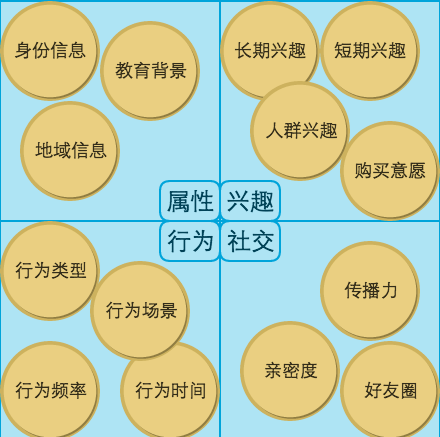
\includegraphics[scale=0.6]{figures/hl_userDimension}}
	      \figcaption{用户画像维度划分}
	      \label{pic:hl_userDimension}
	    \end{figure}
        
        属性维度:属性维度属于传统用户画像的范畴,即对用户的信息进行标签化。一方面,标签化是对用户信息进行结构化,方便计算机的识别和处理;另一方面,标签本身也具有准确性和非二义性,也有利于人工的整理、分析和统计。用户属性指相对静态和稳定的人口属性,例如:性别、年龄区间、地域、受教育程度、学校、公司等信息的收集和建立主要依靠产品本身的引导、调查、第三方提供等,在此基础上需要进行补充和交叉验证。
        \begin{itemize}
        \item 标签来源:不是所有的词都适合充当用户标签,这些词本身应该具有区分性和非二义性;此外,还需要考虑来源的全面性,除了用户主动提供的兴趣标签外,用户在使用的过程中的行为,构建的用户关系等也能够反应用户的兴趣,因此也要将其考虑在内。
        \item 权重计算:得到了用户的兴趣标签,还需要针对用户给这些标签进行权重赋值,用来区分不同标签对于该用户的重要程度。
        \end{itemize}

        兴趣维度:由于用户兴趣维度的重要性,因此有一个独立于用户画像模块的兴趣探索模块,下一章节将会详细介绍到。用户兴趣是更加动态和易变化的特征,首先兴趣受到人群、环境、热点事件、行业等方面的影响,一旦这些因素发生变化,用户的兴趣容易产生迁移;其次,用户的行为多样且碎片化,不同行为反映出来的兴趣差异较大,在用户画像建模的过程中,主要考虑如下几个方面:
        \begin{itemize}
        \item 时效性:随着时间的变化,用户的兴趣会发生转移,有些兴趣会贯穿用户使用社交媒体的全过程,而有些兴趣则是受热点时间、环境因素等的影响。
        \item 长尾性:对于电商领域来讲,那些冷门的用户兴趣的总和可以和那些为数不多的大众化兴趣所占的市场份额相匹配或胜出。
        \item 兴趣和购买意愿的区分:用户具有某方面的兴趣,只代表了他愿意接受这方面的信息,并不能代表他具有购买相关内容的意愿。例如对于一些只看不买的用户,我们认为其购买意愿很小,因此对其会尽可能多的展示免费主题。
        \end{itemize}

        社交维度:如果将主题应用平台的用户视作节点,用户之间的关系视作节点之间的边,那么这些节点和边将构成一个社交的网络拓扑结构,或称作社交图谱。消费信息就是在这个图谱上进行传播。从社交的维度建立用户画像,需要从不同的角度细致和全面地描述这个消费图谱的特征,反应影响信息传播的各层面上的因素,寻找节点之间的关联度,以及刻画图谱本身的结构特征。其中包括:
        \begin{itemize}
        \item 用户个体对消费信息传播的影响:不同用户在信息传播过程中的重要性不一样,影响大的用户对于信息的传播较影响小的用户更具有促进作用。
        \item 量化用户关系紧密度:存在社交关联的用户,关系越近的用户之间越容易产生相同的消费行为。
        \item 寻找相似的用户:消费中非对等的关系本身可以认为是一种认证,用户基于兴趣、消费态度等原因反应到线上的一种关联。那么在消费维度上的相似用户至少能反应他们在某种因素上的一致性。
        \item 识别关系圈:从关系图谱的本身的结构出发,从中发掘关联紧密的群体,有助于促销广告的精准投放和主题包的推广。以上关于关系建模的任务可以看作是逐步深入的,从“个体”-->“关联”-->“相似”-->“群体”的逐渐深入。
        \end{itemize}

        行为维度:分析用户的行为,建立行为模式有两个任务:针对典型个体行为进行时序分片,分析用户成长的相关因素;针对典型群体的行为进行统计,为其构建通用的用户画像。
        \begin{itemize}
        \item 典型个体的行为时序分析。所谓典型个体是指某段时间内,成长比较突出的用户。例如从一个新用户从新注册到点击过百、浏览过千需要有一个积累过程,有些用户积累较快,有些较慢,而这些积累较快的用户可以作为典型个体;或者某些用户在某一阶段消费有限,但在某时刻消费激增,无论是消费金额还是数量都变化很大,这种也可以作为典型个体。针对典型个体,需要挖掘与其用户成长相关的行为因素。基本方法是对时间进行分片,获取用户在不同时间片上的行为统计,以及在各个时间分片上的用户成长指标(点击量、购买量、点击转换比等)。在此基础上针对用户行为的统计量的变化,利用关联性分析或回归来分析用户成长与哪些因素有关。
        \item 典型群体行为模式分析。针对典型个体,从用户的基本信息、人口信息、兴趣维度,可以将相似的典型用户划分为同一的群体,称作典型群体,针对典型群体中的用户按照成长程度进行划分,按不同的成长阶段统计用户行为,即建立了该典型群体的行为模型。例如,对于“年龄在20~30岁,女性,付费用户”这样的典型群体,从日点击量、月消费额等维度将其划分到初创、成长、快速提升、成熟等阶段,针对不同成长阶段内的行为组合进行统计,结果构成该群体的行为模式。如\autoref{pic:hl_usergroup}
        \end{itemize}

        \begin{figure}
        \centering
          \framebox{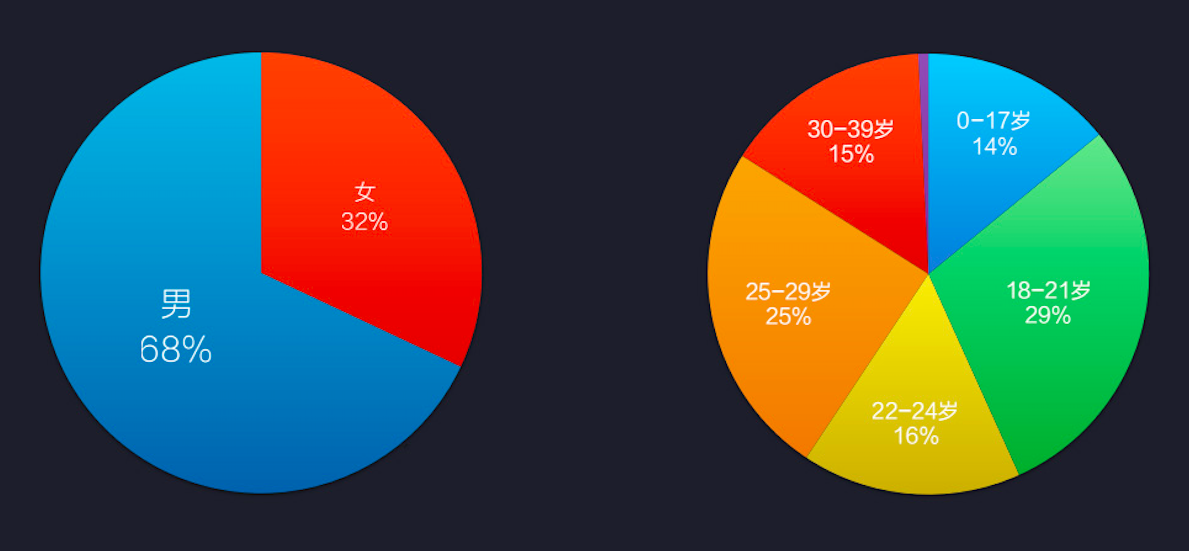
\includegraphics[scale=0.35]{figures/hl_usergroup}}
          \figcaption{电子商务市场用户群体分布}
          \label{pic:hl_usergroup}
        \end{figure}

		\subsection{用户画像应用场景}
		优化电子商务市场供求:改变了原有的先设计、再销售的传统模式。第三方主题设计师在设计一款新产品前,会先设定好主题类型,然后通过用户画像平台中分析该用户群体的偏好,有针对性的设计产品,从而改变原先新产品高失败率的窘境,增强销售表现。如设计一款智能手表主题,面向28-35岁的年轻男性,通过在平台中进行分析,发现属性=“金属”、风格=“硬朗”、颜色="深灰色"、价格区间=“中等”的偏好比重最大,那么就给新产品的设计提供了非常客观有效的决策依据。
		
		提高新人留存率:工商管理有一个理论叫做,维护一个老用户的成本是获取新用户成本的五分之一甚至更低。所以如果能够把一些已经流失的用户召回来,这时候成本比拉一个新用户低得多,你做的事也会带来更大的价值。鉴于此公司启动了一个项目叫"用户画像之拉新",首先利用用户画像得出最近一个月没有登录过的用户数据,然后根据浏览时长分档,这是因为用户需要花自己的时间成本才能留下的最有价值的标签,之后利用用户静态标签,像姓名、职业、年龄、地域分布做进一步的细分,最后针对不同类型的用户提供不同的优惠活动。ABtest显示,与传统一刀切的推荐相比,基于用户画像的拉新留存率提高了约50\%。
		
		用户消费等级分群:大至用户终端品牌、机型、操作系统,细至屏幕分辨率、屏幕尺寸,用户画像记录了每一个用户群体的详细终端特征。哪一类人群最容易被这款应用吸引,愿意为这款应用付费?开发者经常考虑的问题可以从用户画像找到答案。每一个用户群的价格分布、增值业务费用分布以及流量费用,包括用户详细的消费特征,比如付费频率,丰富了推荐系统的数据依据。
		
		用户流失预警:一般情况用户在消费过程中会经历对如下几个期间:新鲜期,沉迷期,消退期,离开四个阶段,如何能够延长用户在应用的停留周期是需要解决的问题之一。用户画像可以辅助推荐系统进行流失用户特征分析,通过决策数算法,分析流失用户特征,建立不同原因流失的用户模型,然后通过这些特征得到当前在应用活跃用户中匹配流失概率高的用户数据。
		
		反作弊:用户画像会对用户的消费能力、空闲时间、信用评级等维度进行打分;利用反作弊模型通过业务方访问收集数据,供安全部门参考。

	\section{推荐系统用户兴趣探索}
		现实世界的一切事物都处在变化之中。用户的兴趣、物品的属性都是在不断的变化,一个系统中每天会有大量的新用户新物品加入;时间作为一种重要的上下文信息(Context),不同的时间用户也会有不同的兴趣,比如用户在白天和晚上的兴趣可能不同,周末和工作日的兴趣可能不同,不同的季节用户的兴趣也会有所不同。因此,合理的利用时间信息,对推荐的精准度和用户的满意度将会有很大的提升。而传统的推荐系统在设计时并没有主动的考虑到时间因素,推荐系统的动态效应表现在:
		\begin{itemize}
		\item 用户偏好随时间变化(User bias shifting):用户可能在某一天只对他喜欢的物品评分,某一天可能只对他不喜欢的物品评分。因此用户某一天的平均分是随时间变化的。
		\item 物品偏好随时间变化(Item bias shifting):物品的受欢迎程度也是随时间变化的。一款主题包在刚上线的时候的因为用户关注度小平均评分会很高,随着时间的推移,越来越多的用户参与到评分中,会使其慢慢接近真实的评分。
		\item 用户兴趣随时间变化(User preference shifting):用户在不同的时候可能有不同的兴趣,比如小孩都喜欢动漫主题包,但当他长大了可能喜欢汽车主题包。
		\item 季节效应:用户行为会受季节效应的影响。主题推荐中主要的季节效应有暑期的效应,以及一些纪念日的效应(比如国庆纪念日前后,抗日题材的主题包会受到较多的关注)。
		\end{itemize}

		为保持推荐系统的动态特性,工业界一般用数据追加的方式进行增量计算。推荐系统利用hadoop集群可以在2个小时内完成最近24小时数据的增量计算并将结果追加到现有的计算结果中,耗费的这2个小时可以用更少的时间进行增量计算并做数据追加。

		\subsection{用户行为数据存储}
		电子商务用户行为数据的特点包括:用户基数庞大。以电子商务网站淘宝网为例,注册用户往往以千万计,活跃用户达百万计;用户规模增长快。每个用户的行为数量较小。即使是活跃用户,每天最多也只能产生上百条行为记录,每年不超过十万条;用户行为的计算较为复杂。计算用户的两次登录间隔天数、反复购买的商品、累积在线时间,这些都是针对用户行为的计算,通常具有一定的复杂性;用户行为数据格式不规整,字段丢失率较高。根据用户行为数据的这些特点采用基于Hadop分布式的架构。

		\subsection{用户行为数据预处理}
		Hive是建立在Hadoop上的数据仓库基础架构。它提供了一系列的工具,用来进行数据提取、转换、加载,是一种可以存储、查询和分析存储在Hadoop中的大规模数据机制。可以把Hadoop下结构化数据文件映射为一张成Hive中的表,并提供类sql查询功能,除了不支持更新、索引和事务,sql其它功能都支持。可以将sql语句转换为MapReduce任务进行运行,作为sql到MapReduce的映射器。提供shell、JDBC/ODBC、Thrift等接口。优点是成本低可以通过类sql语句快速实现简单的MapReduce统计。作为一个数据仓库,Hive的数据管理按照使用层次可以从元数据存储、数据存储和数据交换三个方面介绍。数据预处理是数据挖掘过程中一个重要步骤,当原始数据存在不一致、重复、含噪声、维度高等问题时,更需要进行数据的预处理,以提高数据挖掘对象的质量,最终达到提高数据挖掘所获模式知识质量的目的。
		
		随着电子商务市场交易规模的逐步增大,积累下来的业务数据和用户行为数据越来越多,这些用户数据往往是电子商务平台最宝贵的财富。目前在电子商务推荐系统中大量地应用到了机器学习和数据挖掘技术,例如个性化推荐、搜索排序、用户画像建模等等,为企业创造了巨大的价值。数据预处理主要工作是:
		\begin{itemize}
		\item 从原始数据,如文本、图像或者应用数据中清洗出特征数据和标注数据
		\item 对清洗出的特征和标注数据进行处理,例如样本采样,样本调权,异常点去除,特征归一化处理等过程。最终生成的数据主要是供模型直接使用。
		\end{itemize}
		根据不同业务数据的预处理方式也不同,一般来讲原始服务器日志数据脏数据的形成原因包括:缩写词不统一,数据输入错误,不同的惯用语,重复记录,丢失值,不同的计量单位,过时的编码等。相应的,数据预处理内容包括数据清理、数据集成、数据变换、数据归约、数据离散化。数据清理包括格式标准化、异常数据清除、错误纠正、重复数据的清除。对于电子商务用户数据来讲,引起空缺值的原因主要是用户设备异常造成的,有些时候是因为与其他已有数据不一致而被删除或数据的改变没有进行日志记载。根据数据空缺情况的不同有不同的处理方式:
		\begin{itemize}
		\item 忽略元组。当一个记录中有多个属性值空缺、特别是关键信息丢失时,已不能反映真实情况,它的效果非常差。
		\item 去掉属性。缺失严重时,已无挖掘意义。
		\item 人工填写空缺值。但是工作量大且可行性低。
		\item 默认值。比如使用unknown或-∞。
		\item 使用属性的平均值填充空缺值。
		\item 预测最可能的值填充空缺值。使用贝叶斯公式或判定树这样的基于推断的方法。
		\end{itemize}

		\subsection{用户行为建模}

		实体域。当我们想基于用户行为分析来建立用户兴趣模型时,我们必须把用户行为和兴趣主题限定在一个实体域上。个性化推荐落实在具体的推荐中都是在某个实体域的推荐。对于手机主题应用市场来说,实体域包括所有的主题,背景图片,铃声,闹铃等。  用户行为。浏览,点击,下载,试用,购买,评论等都可是用户行为。本文所指的用户行为都是指用户在某实体域上的行为。比如用户在手机铃声产生的行为。用户兴趣。用户的兴趣维度,同样是限定在某实体域的兴趣,通常以标签+权重的形式来表示。比如,对于手机主题,用户兴趣向量可以是「动漫,0.6」,「体育,0.1」,「情感,0.7」等分类标签。值得一提的是,用户兴趣只是从用户行为中抽象出来的兴趣维度,并无统一标准。而兴趣维度的粒度也不固定,如「体育」,「电影」等一级分类,而体育下有「篮球」,「足球」等二级分类,篮球下有「NBA」,「CBA」,「火箭队」等三级分类。我们选取什么粒度的兴趣空间取决于具体业务模型。
		
		实际应用中,在社交网络用户的行为一般是主动进行的,例如,自行定义或选择标签,浏览页面,使用站内产品或第三方APP,发表博文或对其他博文内容的点赞或收藏,关注其他用户并将其关注的对象划分到自行设置的各用户组内等。而上述这些社交网络用户的行为能够在一定程度上反映出用户的兴趣。因此,社交网络中,可以根据用户的这些网络行为来进行用户的兴趣挖掘。该阶段是用户行为数据进行建模,以抽象出用户的标签,这个阶段注重的应是大概率事件,通过数学算法模型尽可能地排除用户的偶然行为。基于用户标签的兴趣挖掘方法。具体地,可以根据标签的具体内容,将标签归类到相应的兴趣类别后,再根据用户的自定义标签及其所属的兴趣类别,分析出用户的兴趣。

	\section{本章小结}
	本章首先从学术研究和商业应用两个角度介绍了推荐系统常用的算法,包括协同过滤、聚类算法等若干种不同的推荐算法。然后重点介绍推荐系统用户画像,包括用户画像的构建和用户画像构建标签维度的划分和用户画像诸多应用场景。最后介绍了用户兴趣探索,包括用户行为数据的存储,用户行为数据的预处理和用户行为建模。